\chapter{Implementierung}
Dieses Kapitel umfasst die Implementierung des Distanzvektor-Algorithmus und eine Beschreibung des Quellcodes. Das Projekt ist auf zwei ausführbare Dateien aufgeteilt. Die Hauptdatei mit dem Namen \verb|distance_vector_sim| beinhaltet den als Controller bezeichneten Teil. Der zweite Teil ist ein Programm namens node. Dieses stellt einen Netzwerkknoten dar und wird duch den Controller gestartet. Die Knoten können zwar auch manuell gestartet werden, das ist jedoch mit deutlich mehr Aufwand verbunden, da dann der Nutzer einen sinnvollen Netzwerkgraphen selbst erstellen muss und die entsprechenden Nachbarknoten manuell an jeden Knoten übergeben.

\section{Controller}
Der Controller agiert als Ausgangspunkt und ist für das Starten und Beenden der Knoten verantwortlich. Der dazugehörige Code befindet sich im gleichnamigen Unterverzeichnis des src-Verzeichnisses. Der Controller besteht aus einer Main-Funktion und zwei in die Datei utils.cpp ausgelagerte Funktionen. Am Beginn des Controllers werden alle Parameter für die Kommandozeile mit ihren Standardwerten initialisiert. Danach werden mithilfe der Bibliothek CLI11 die übergebenen Parameter gelesen.\footcite{cli} Sollte eine Konfigurationsdatei angegeben sein, wird diese im nächsten Schritt abgearbeitet, wobei die Werte der Konfigurationsdatei jene der Kommandozeile überschreiben. Dieses Verhalten ist gewollt und erwartet. Die JSON-Datei wird durch die Bibliothek JSON for Modern C++ bearbeitet.\footcite{json} Im Codebeispiel \ref{lst:cmd_args} ist die Initialisierung der Parameter und die Angabe mittels der Bibliothek CLI11 dargestellt.

\begin{minipage}{\linewidth}
\begin{lstlisting}[language={C++}, caption={Angabe der Kommandozeilenparameter}, label={lst:cmd_args}]
bool use_logging{false};
bool log_level_debug{false};
bool simulate_error{false};
size_t node_cnt{7};
string config_file{"N/A"};

const char node_program[7]{"./node"};

app.add_option("node count", node_cnt, "Total number of nodes. Must be > 0.")->check(CLI::PositiveNumber);
CLI::Option* log_flag{app.add_flag("-l, --log", use_logging, "Write log file dist_sync_log.log.")};
app.add_flag("-d, --debug", log_level_debug, "Set log level to debug.")->needs(log_flag);
app.add_option("-f, --file", config_file, "Path to json config file.")->check(CLI::ExistingFile);
app.add_flag("--failure", simulate_error, "Simulate failure of one connection");
\end{lstlisting}
\end{minipage}
Wenn die Parameter sowohl aus der Datei als auch von der Kommandozeile gelesen und übernommen wurden, werden die Einstellungen für das Logging gesetzt. Dabei wird die Bibliothek spdlog verwendet. Ein sogenannter rotating-file-logger wird als Standard-Logger gesetzt und das Log-Level wird den übergebenen Parametern angepasst.

Der nächste Schritt ist das Erstellen des Netzwerkgraphen. Hierfür wird ein einfacher Algorithmus verwendet, welcher versucht, jeden Knoten mit mindestens einem anderen zu Verbinden. Um sicherzustellen, dass ausreichend Verbindungen erstellt werden, ist die Anzahl der Kanten auf zwei mehr als die Anzahl der Knoten festgelegt. Die Funktion für das Erstellen befindet sich in der Datei utils.cpp. In der dazugehörigen Header-Datei ist auch ein C++-Struct, welches alle Informationen zu einem Knoten speichert. Wenn der Netzerkgraph erstellt ist, wird in einer Schleife ein Vektor mit den Einträgen für die Knoten befüllt. Identifiziert werden die Knoten einerseits über eine Nummer, die auch ihrem Index in diesem Vektor entspricht, andererseits auch über ihre Portnummer. Die Portnummern werden beginnend mit 9900 aufsteigend zugewiesen. Der erste Knoten erhält somit die Nummer 9900, der zweite die Nummer 9901 und so weiter. Ist die Option für die Simulation eines Verbindunsausfalls gesetzt, wird im nächsten Abschnitt festgelegt, welche Verbindung ausfällt. Hierfür wird ein zufälliger Knoten ausgewählt. Von diesem Knoten wird sein erste Nachbar aus der Liste gewählt. Die Verbindung zwischen diesen beiden Knoten wird dann als fehlerhaft gekennzeichnet.

Sind alle Einstellungen gesetzt beginnt das eigentliche Erstellen der Knoten. Dafür werden in einer Schleife die Kommandozeilenparameter der Knoten in einem Vektor gespeichert. Der erste Parameter ist der Name des Programms, in diesem Fall \verb|./node|. Von dieser Zeichenkette wird ein Zeiger auf das erste Zeichen in einem Vektor gespeichert. Die nächsten beiden Parameter sind die Indikatoren für das Logging, welche analog zu denen des Controllers gesetzt werden. Danach folgt der Port des Knoten, welcher mit der Option -p übergeben wird. Nach dem eigenen Port folgen jene Ports der direkten Nachbarn. Jeder Knoten erhält mit der Option -n die Portnummern seiner Nachbarn. Die letzte Option wird nur gesetzt, wenn zuvor dieser Knoten als fehlerhaft deklariert wurde. In Zeile 22 und 23 des Codebeispiels \ref{lst:node_create} sieht man, dass dem Knoten mit der Option --failure der Port übergeben wird, zu dem ein Verbindungsfehler simuliert wird. Der letze Schritt ist das eigentliche Starten der Knoten. Hierfür wird wie in Zeile 28 des Code-Ausschnitts zu sehen sit ein neuer Prozess erstellt. In diesem Prozess wird mittels execv  das Programm node ausgeführt.

\begin{lstlisting}[language={C++}, caption={Erstellen der Knoten}, label={lst:node_create}]
for (size_t i{0}; i < node_cnt; i++) {
    vector<char*> node_cmd_args;
    node_cmd_args.push_back((char*)"./node");
    
    if (use_logging) {
        node_cmd_args.push_back((char*)"--log");
        if (log_level_debug) {
            node_cmd_args.push_back((char*)"--debug");
        }
    }
    
    node_cmd_args.push_back((char*)"-p");
    node_cmd_args.push_back(&nodes[i].port[0]);
    
    if (network[i].size() > 0) {
        node_cmd_args.push_back((char*)"-n");
        for (size_t j{0}; j < network[i].size(); j++) {
            node_cmd_args.push_back(&nodes[(network[i][j])].port[0]);
        }
    }
    if (nodes[i].failure) {
        node_cmd_args.push_back((char*)"--failure");
        node_cmd_args.push_back(&nodes[i].failed_connection[0]);
    }
    node_cmd_args.push_back(NULL);
    nodes[i].cmd_args = node_cmd_args;

    nodes[i].pid = fork();
    if (nodes[i].pid == -1) {
        spdlog::error("Creating node process {} failed.", i);
    } else if (nodes[i].pid> 0) {
        fmt::print("[{}] Create node process with pid {}.\n", format(fg(fmt::color::magenta), "Controller"), nodes[i].pid);
        spdlog::info("Create node process with pid {}.", nodes[i].pid);
    } else {
        char** node_argv{node_cmd_args.data()};
        execv(node_program, &node_argv[0]);
        perror("execl");
        exit(EXIT_FAILURE);
    }
}
\end{lstlisting}

Sobald die Knoten erstellt sind, sind alle Aufgaben des Controllers erfüllt und er wartet nur noch auf einen Keyboard-Interrupt, bei welchem er die Prozesse der Knoten beendet.

\section{Knoten}
Das Programm des Knoten ist jener Teil, der den Algorithmus implementiert. Das Programm ist unter dem Namen node aufrufbar und besteht aus insgesamt drei Klassen und einer Main-Funktion. In dieser werden nur die Parameter der Kommandozeile ausgelesen und gespeichert. Dies geschieht gleich wie im Controller und wird daher nicht weiter erläutert. Der relevante Teil beginnt mit dem Aufruf der Methode run der Node-Klasse. Um einen Überblick über die einzelnen Klassen und deren Beziehungen zu erhalten ist in Abbildung \ref{fig:class_diag} ein Klassendiagramm dargestellt.

\begin{figure}
    \centering
    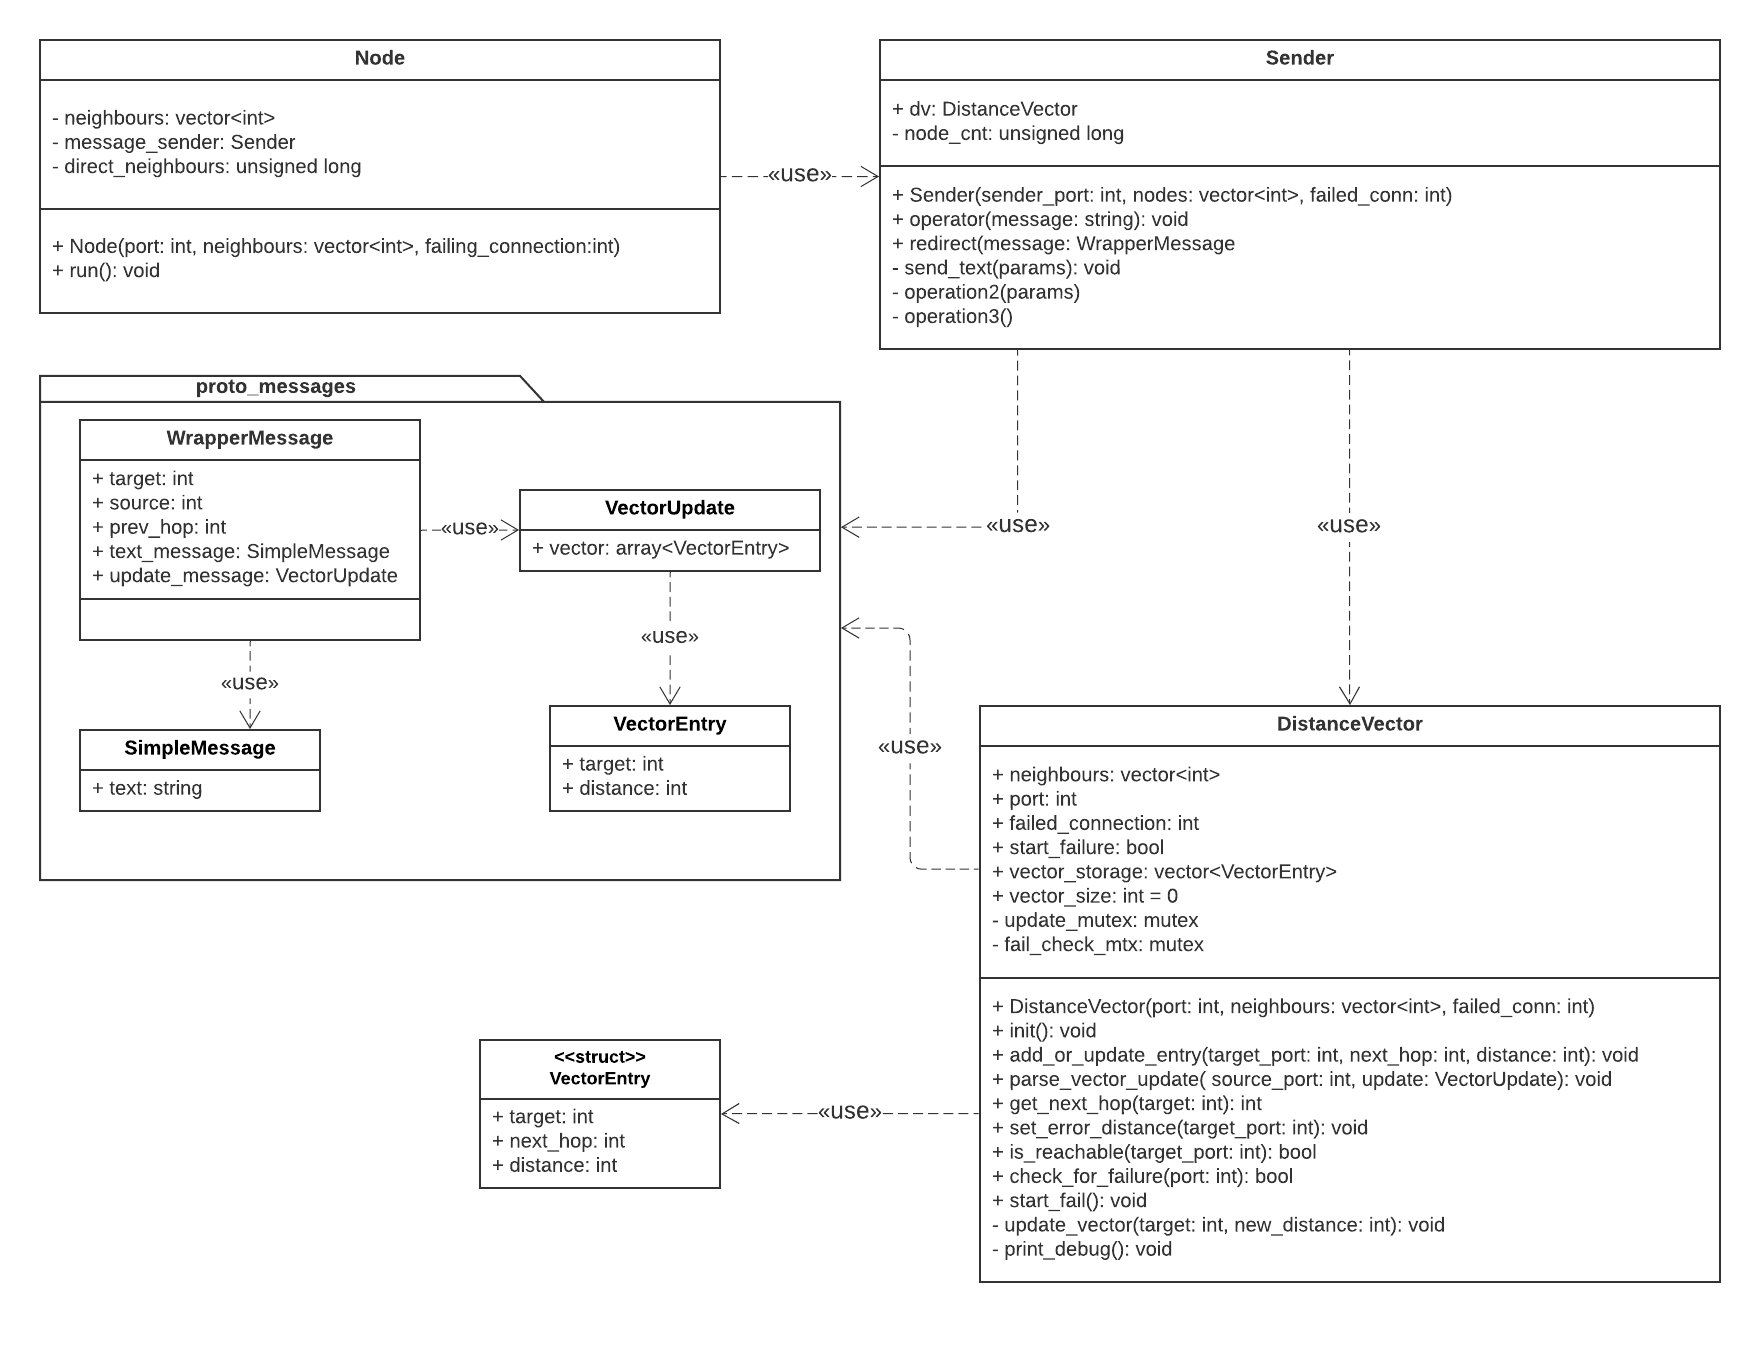
\includegraphics[width=\textwidth]{images/nvs_class_diag.png}
    \caption{Klassendiagramm des node-Programms}
    \label{fig:class_diag}
\end{figure}

\subsection{Node-Klasse}
Diese Klasse dient als Hülle für alle weiteren Klassen und beinhaltete somit die gesamte Logik. Die Klasse hat nur zwei Methoden. In der run-Methode wird ein Socket erstellt und in einer Endlosschleife auf neue Verbindungen gewartet. Ist eine Verbindung dieses Knotens als fehlerhaft gekennzeichnet, wird außerdem ein Thread gestartet, welcher nach einer Verzögerung von 30 Sekunden die Simulation des Fehlers startet. Dabei wird eine Variable gesetzt, welche beim Verbindungsaufbau abgefragt wird. Wird eine Verbindung zum Socket aufgebaut, wird der Socket an einen neu erstellten Thread weitergegeben, welcher die Verbindung bearbeitet. Der Thread führt die zweite Methode der node-Klasse aus, \verb|serve_request|. Hier wird die eingehende Nachricht gelesen und zur Bearbeitung weitergegeben. Ist es eine Textnachricht, wird ihr Inhalt auf der Kommandozeile ausgegeben. Handelt es sich um eine Vektor-Aktualisierung, wird diese von der DistanceVector-Klasse bearbeitet. Die letzte Option ist, dass die Nachricht nur weitergeleitet werden muss. In diesem Fall wird sie an die redirect-Methode der Sender-Klasse übergeben. Im Codebeispiel \ref{lst:serve_request} ist die Methode zum Bearbeiten einer Verbindung angegeben. Je nach Art der Nachricht wird anders mit ihr verfahren.

\begin{lstlisting}[language={C++}, caption={Bearbeiten einer Verbindung}, label={lst:serve_request}]
asio::streambuf buf;
asio::read_until(sock, buf, '\n');
proto_messages::WrapperMessage message;
istream is{&buf};
message.ParseFromIstream(&is);
if (message.target() == this->message_sender.dv.port) {
    if (message.has_text_message()) {
        fmt::print("[{}] ({}) Received: " 
        + message.text_message().text() + "\n"
        , format(fg(fmt::color::cyan)
        , "Node " + to_string(this->message_sender.dv.port))
        , format(fg(fmt::color::pale_green), "TextMessage"));
        spdlog::info("Received message: '{}'"
        , message.text_message().text());
    } else if (message.has_update_message()) {
        this->message_sender.dv.parse_vector_update(
            message.source(), message.update_message());
    }
} else {
    this->message_sender.redirect(message);
}

sock.close();
\end{lstlisting}

\subsection{Protobuf-Klassen}
Dieser Abschnitt befasst sich mit den Nachrichten, welche mit der Protocol-Buffer-Bibliothek erstellt werden. Google Protocoll Buffers ist eine Bibliothek zum Serialisieren und Deserialisieren von Daten. Für die Implementierung des Distanz-Vektor-Algorithmus werden insgesamt vier Nachrichten verwendet. Zu besseren Lesbarkeit sind in den folgenden Sekionen die Datentypen meist nicht angegeben. Ist kein Datentyp angegeben, so handelt es sich um einen 32-Bit Integer.
\subsubsection{WrapperMessage}
Um das Deserialisieren zu vereinfachen, sind die eigentlichen Nachrichten in eine Wrapper-Nachricht namens WrapperMessage verpackt. Diese enthält neben der eigentlichen Nachricht noch drei Felder für das Ziel, den Herkunftsknoten und den zuletzt besuchten Knoten. In dieser Verpackungs-Klasse sind eine der beiden folgenden Klassen gespeichert. 
\subsubsection{SimpleMessage}
Die erste Nachrichten-Klasse ist SimpleMessage, welche nur ein Feld, eine Zeichenkette enthält. Diese Nachricht dient als Testnachricht und soll die in einem echten Netzwerk versendeten Nutzdaten simulieren. 
\subsubsection{VectorUpdate}
Die Klasse VectorUpdate versendet die Routing-Informationen. Sie enthält eine Liste von Einträgen der Klasse VectorEntry, eine in diese Nachricht eingebettete Nachricht. Jeder dieser Einträge repesentiert einen Eintrag in der Weiterleitungstabelle des Sender-Knotens und hat daher zwei Felder, eines für das Ziel und eines für die Distanz zu diesem.

\subsection{Sender-Klasse}
Die Sender-Klasse ist, wie der Name schon sagt, für das Senden von Nachrichten über das Netzwerk verantwortlich. Sie ist in der Node-Klasse gespeichert. Sie beinhaltet zusätzlich zu den Funktionen zum Senden auch die DistanceVektor-Klasse. Die Klasse wird als Thread ausgeführt, welcher periodisch in zufälligen Zeitabschnitten von 8 bis 12 Sekunden Nachrichten aussendet. Bevor das Aussenden der Nachrichten beginnt, wird die DistanceVector-Klasse mit ihrer Methode init initialisiert.

Nach der ersten Hälfte des Intervalls wird eine Vektor-Aktualisierung an alle Nachbarknoten versendet. Dafür wird die Methode \verb|send_update_to_neighbours| aufgerufen, welche wiederum die Funktion \verb|send_update| für jeden Nachbarknoten aufruft. Dabei wird eine neune Instanz der WrapperMessage angelegt und mit den in der Weiterleitungstabelle vorhandenen Einträgen befüllt. Ist die zweite Hälfte des Intervalls verstrichen, wird eine SimpleMessage an alle bekannten Knoten, nicht nur an alle Nachbarn ausgesendet. Dieser Vorgang wiederholt sich in einer Endlosschleife.

Die Methode redirect zum Weiterleiten einer Nachricht ist ebenfalls Teil dieser Klasse. Ihr wird eine WrapperMessage als Parameter übergeben. In der Weiterleitungstabelle wird nach dem nächsten Knoten gesucht, an den die Nachricht gesendet werden muss, um zum Ziel zu gelangen. Ist der Knoten gefunden, wird eine neue Verbindung geöffnet und die Nachricht versendet. 

Vor jedem Versenden einer Nachricht, unabhängig davon, ob dies nur Weiterleiten oder das Versenden einer neuen Nachricht ist, wird überprüft, ob die zum nächsten Knoten noch besteht. Diese Übrprüfung bezieht sich auf den simulierten Ausfall und ist keine tatsächliche Überprüfung der Erreichbarkeit. Ist die Verbindung als fehlerhaft gekennzeichnet, wird in der Weiterleitungstabelle der Wert für Unendlich, in dieser Implementierung das Maximum eines 16-Bit Integers, eingetragen.

\subsection{DistanceVector-Klasse}
Diese Klasse beinhaltet die eigentliche Implementierung des Algorithmus. Das Herzstück ist ein Vektor des Structs VectorEntry. In diesem wird für jeden bekannten Knoten seine Portnummer, der nächste Knoten, über den er erreicht werden kann und die Distanz zu ihm gespeichert. Dieser Vektor wird von der Mehtode \verb|add_or_update_entry| bearbeitet. Die Methode erhält als Parameter den Ziel-Port, den nächsten Hop und die Distanz. Zuerst wird überprüft, of es sich bei dem Ziel um den Knoten selbst handelt. In diese Fall wird nichts geändert.